\subsection{\ainterface}
\label{sec:admininterface}
The \admin[] interface is illustrated in figure \ref{fig:admin_interface}.
After login, the \admin[] is presented with the \textit{main} window. All the window have a back function which enables the \admin[] to return to the previous window.

\subsubsection{Main}
The ``Main'' \admin window gives access to administration options and the functionality from the \astaff and \aclient main windows. The window contains: 
\begin{itemize}
	\item The button ``Administrate departments, categories, and tags'' which directs the \admin[] to the ``Department Administration'' window.  
	\item The button ``Administrate persons'' directs the \admin[] to the ``Person Administration'' window.
\end{itemize}
plus the buttons from the \astaff[] and \aclient[] ``main'' window.
%The ``Main'' administrator window contains two new  and ``Administrate persons''. The buttons from the ``Main'' \astaff and \aclient window are also shown.  

\subsubsection{Person administration}

\subsubsection{Department administration}

\subsubsection{Person view}

\subsubsection{Category view}

\subsubsection{Tag view}



\begin{comment}

The \ainterface[] is an extension of the \sinterface[], as the \ainterface[] is entered through the \sinterface[].
This makes sense because all persons given the permissions to enter the \ainterface[], will also be \astaff[] members.
There are two major fields\fixme{Foretr\ae kker noget andet her. M\aa{}ske bare classes?} of which the \admin[] has influence on, departments and persons.
These two are described in the following.

\subsubsection{Administrate Persons}
When an \admin[] enters the administrate persons window he/she is presented with a list of persons and a ``New Person'' button.
From this window the \admin[] can select an existing person and change the data of him or her 

\subsubsection{Administrate Departments}

\end{comment}


\begin{figure}[H]
	\centering
		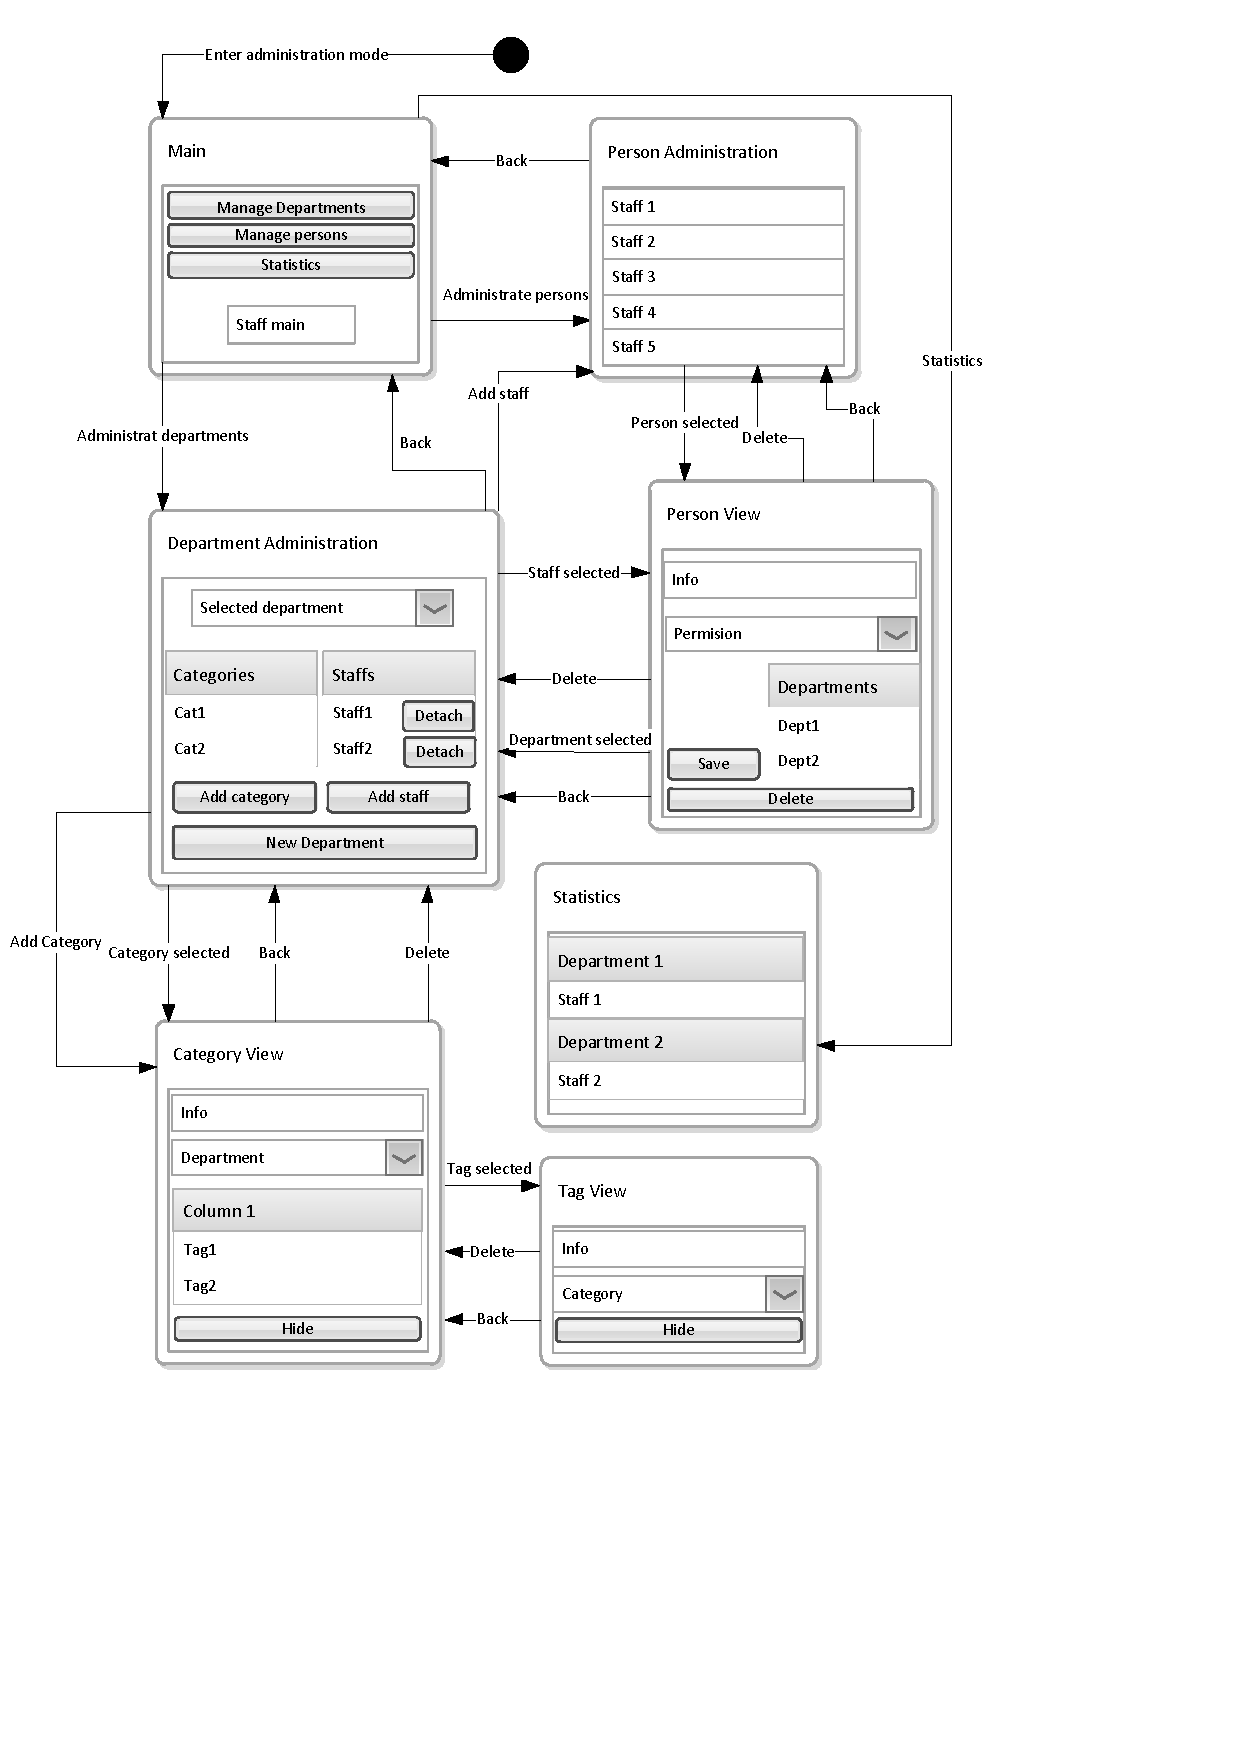
\includegraphics[width = \textwidth, clip=true, trim=0 5cm 3cm 0]{input/application_domain_analysis/Navigation_DiagramAdmin.pdf}
	\morscaption{\ainterface[c]}
	\label{fig:Navigation_DiagramAdmin}
\end{figure}

\begin{comment}
\begin{itemize}
	\item department, including:
	\begin{itemize}
		\item categories
		\item tags
	\end{itemize}
	\item persons
\end{itemize}
\end{comment}